\documentclass{article}\usepackage[]{graphicx}\usepackage[]{color}
%% maxwidth is the original width if it is less than linewidth
%% otherwise use linewidth (to make sure the graphics do not exceed the margin)
\makeatletter
\def\maxwidth{ %
  \ifdim\Gin@nat@width>\linewidth
    \linewidth
  \else
    \Gin@nat@width
  \fi
}
\makeatother

\definecolor{fgcolor}{rgb}{0.345, 0.345, 0.345}
\newcommand{\hlnum}[1]{\textcolor[rgb]{0.686,0.059,0.569}{#1}}%
\newcommand{\hlstr}[1]{\textcolor[rgb]{0.192,0.494,0.8}{#1}}%
\newcommand{\hlcom}[1]{\textcolor[rgb]{0.678,0.584,0.686}{\textit{#1}}}%
\newcommand{\hlopt}[1]{\textcolor[rgb]{0,0,0}{#1}}%
\newcommand{\hlstd}[1]{\textcolor[rgb]{0.345,0.345,0.345}{#1}}%
\newcommand{\hlkwa}[1]{\textcolor[rgb]{0.161,0.373,0.58}{\textbf{#1}}}%
\newcommand{\hlkwb}[1]{\textcolor[rgb]{0.69,0.353,0.396}{#1}}%
\newcommand{\hlkwc}[1]{\textcolor[rgb]{0.333,0.667,0.333}{#1}}%
\newcommand{\hlkwd}[1]{\textcolor[rgb]{0.737,0.353,0.396}{\textbf{#1}}}%

\usepackage{framed}
\makeatletter
\newenvironment{kframe}{%
 \def\at@end@of@kframe{}%
 \ifinner\ifhmode%
  \def\at@end@of@kframe{\end{minipage}}%
  \begin{minipage}{\columnwidth}%
 \fi\fi%
 \def\FrameCommand##1{\hskip\@totalleftmargin \hskip-\fboxsep
 \colorbox{shadecolor}{##1}\hskip-\fboxsep
     % There is no \\@totalrightmargin, so:
     \hskip-\linewidth \hskip-\@totalleftmargin \hskip\columnwidth}%
 \MakeFramed {\advance\hsize-\width
   \@totalleftmargin\z@ \linewidth\hsize
   \@setminipage}}%
 {\par\unskip\endMakeFramed%
 \at@end@of@kframe}
\makeatother

\definecolor{shadecolor}{rgb}{.97, .97, .97}
\definecolor{messagecolor}{rgb}{0, 0, 0}
\definecolor{warningcolor}{rgb}{1, 0, 1}
\definecolor{errorcolor}{rgb}{1, 0, 0}
\newenvironment{knitrout}{}{} % an empty environment to be redefined in TeX

\usepackage{alltt}

\usepackage{geometry}
\geometry{verbose,tmargin=2cm,bmargin=2.2cm,lmargin=2.5cm,rmargin=2.5cm}

\usepackage{url}
\usepackage{breakurl}
\usepackage[parfill]{parskip}
\usepackage{amsmath}



\IfFileExists{upquote.sty}{\usepackage{upquote}}{}
\begin{document}
\begin{center}
\section*{Win Forecasting Through Predictive Modeling}
by Travis Byrum
\end{center}
\paragraph
\\
The most important purpose of NBA analytics is player evaluation since player performance is the deciding factor behind team wins.  Determining a player's contribution to team performance is difficult due to basketball's team-oriented nature and as a result there is an great deal of debate on the subject.  A common approach is to use plus/minus metrics as means of evaluating a player's isolated production.  The idea behind plus/minus is to use the net difference in score of a player on versus off the floor as a an indicator of that player's contribution to team performance.  Others have noted that using the pure point differential would be a poor metric in determining a player's impact on team performance since it is heavily influenced by the other players on the court.  This problem led to the creation of other metrics such such as $\textit{APM}$ (Adjusted Plus Minus) which attempts to reduce bias by taking into account teammate and opponent level of talent.  One of the most recent versions of the plus/minus metric is $\textit{RAPM}$ (Regularized Adjusted Plus Minus) which was developed by analyst Jeremias Engelmann as a means of reducing the standard errors of win predictions associated with $\textit{APM}$.  This is accomplished through the use of ridge regression which penalizes unreasonable parameter estimates.  The flexibility of $\textit{RAPM}$ is what makes it so compelling.  The rating can be used to not only evaluate an individual player but also can be combined to forecast lineups and team wins.
\paragraph
\\
The purpose of this article is to attempt to outperform  $\textit{RAPM}$ through the use of predictive modeling.   Although plus/minus approaches are an extremely useful heuristic, it is possible to achieve greater accuracy in forecasting team wins.  To accomplish this, I decided to take a lineup-based approach where the stats from each individual player in the lineup function as the covariates and the lineup-associated wins would be the dependent variable.  In order to take advantage of the wide variety of data types associated with NBA statistics, I used regression decision trees due to their flexibility in modeling interactions.  More specifically, I used an ensemble learning technique known as gradient boosting (also known as $\textit{GBM}$) .  The idea behind gradient boosting is to combine several smaller decision tree models each with individually weak predictive performance, into a larger model with greater performance.  It can be understood as an an additive model \footnote{http://en.wikipedia.org/wiki/Gradient$\textunderscore$boosting} as seen in the following equation:
\begin{equation}
F(x) = \sum_{i=1}^M \gamma_i h_i(x) + \mbox{const}.
\end{equation}
In this context, each term $h_i(x)$ represents an individual regression decision tree and $\gamma_i$ is a weight calculated through resampling .  Although the specifics as to how the weights and terms are derived is a bit complicated, the advantage of this approach is greater predictive accuracy and flexibility than would be achievable with standard OLS regression.
\paragraph
\\
To apply this approach, I decided to fit the model on lineup data from the 2014-2015 season\footnote{Data gathered from Basketball-Reference}.  An individual row of the data includes information on specific lineup combinations, including games/minutes played and net points.  This can be seen in the following output. 
\\
\begin{knitrout}
\definecolor{shadecolor}{rgb}{0.969, 0.969, 0.969}\color{fgcolor}\begin{kframe}
\begin{verbatim}
##   Rk                                                   Lineup  Tm  Season
## 1  1 M. Barnes | B. Griffin | D. Jordan | C. Paul | J. Redick LAC 2014-15
##    G     MP Tm_poss Opp_poss Pace   FG  FGA FGper X3P X3PA X3Pper eFGper
## 1 60 1215.9    2382     2384 94.1 1099 2162 0.508 269  638  0.422  0.571
##    FT FTA FTper  PTS FG_opp FGA_opp FGper_opp X3P_opp X3PA_opp X3Pper_opp
## 1 432 625 0.691 2899    943    2131     0.443     208      572      0.364
##   eFGper_opp FT_opp FTA_opp FTper_opp PTS_opp
## 1      0.491    350     470     0.745    2444
\end{verbatim}
\end{kframe}
\end{knitrout}

\paragraph
\\
The main point of interest is the net points associated with each lineup since this is what largely determines team wins.  I decided to project the net points into win percentages using the formula\footnote{http://statitudes.com/blog/2013/09/09/pythagoras-of-the-hardwood/}:
\begin{equation}
Win\% = \frac{\text{points for}^{13.91}}{\text{points for}^{13.91} + \text{points against}^{13.91}}
\end{equation}
\paragraph
\\
This projection is known as the Pythagorean win expectation.  It can be thought of as the winning percentage of a lineup if they were playing $100\%$ of the team's minutes.  Although we are modeling a wins projection for interpretability, this is the same as modeling the point differential per lineup and then applying a transformation.  Intuitively since we think of lineup production as a function of the individual players' production, I decided to use the individual player stats as predictors.  With this in mind the model formula becomes
\begin{equation}
E(Win\%)_{i}\sim X_{player1i}+X_{player2i}+X_{player3i}+X_{player4i}+X_{player5i}....
\end{equation}
where $i$ corresponds to the $i^{th}$ lineup and $X_{player1i}$ corresponds to a statistic for a player in lineup $i$.  I've included a number of different statistics in the model for each player including evaluation ratings such as $\textit{PER}$ and $\textit{Offensive/Defensive Rating}$.  The final result is a $365$ length vector for each lineup which includes $73$ unique performance metrics for each player.  The idea here is that we can combine information across players' average performances to predict their specific performance in a given lineup combination.  Although many of the variables are very correlated with each other, the beauty of this modeling approach is that boosted decision trees are already robust against collinearity.
\paragraph
\\
Using the previousspecification, I ran the model on $3911$ different lineup combinations from the 2014-2015 season.  This number was chosen by necessity since I did not have the necessary individual statistics for every player in every lineup.  Since the model does not make the familiar probabilistic assumptions of linear regression, there are different diagnostics to determine overfitting.  Since $\textit{GBM}$ are built from a large number of smaller decision trees, one of the most important parameters is determining the number of trees (known as the iterations) to fit the data.  The following plot gives us the squared error loss associated with increasing the number of trees:

\begin{knitrout}
\definecolor{shadecolor}{rgb}{0.969, 0.969, 0.969}\color{fgcolor}

{\centering 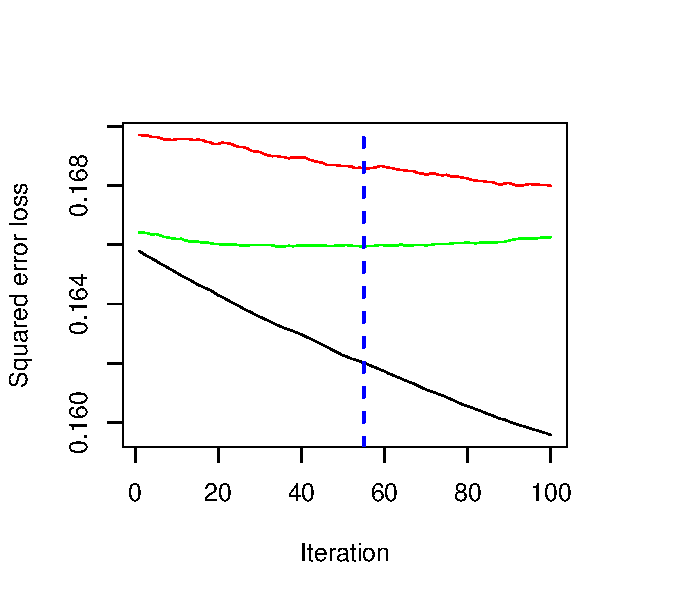
\includegraphics[width=\maxwidth]{figures/unnamed-chunk-2-1} 

}



\end{knitrout}

\paragraph
\\
The squared error loss in this context is calculated from the actual response (lineup win projections calculated from point differentials) against the predicted response with a lower error being better.  The black line indicates the in sample squared error while the red and green lines indicate squared error occurring from $n$-fold cross-validation.  The dotted blue line represents a guess at the optimal number of iterations which achieves a balance between overfitting and predictive power.  Another parameter useful for optimization is known as the learning rate which generally specifies the rate of the model's convergence.  A lower learning rate is regarded as a protection against overfitting at the expense of computation.  After randomly splitting the 2014-2015 lineup data into a training and testing set, I found that $\textit{RAPM}$ derived win projections had a mean squared error of 0.175 versus the model's mean squared error $0.163$ on the training set.
\begin{equation}
\mathbf{MSE}_{RAPM}=0.175\left |  \right |\mathbf{MSE}_{Model}=0.163
\end{equation}


\paragraph
\\
The real test of the model's predictive power, is using it to predict lineup winning percentages in future seasons.  To do this I predicted winning percentages on a test dataset of $n=978$ \footnote{Data gathered from Basketball-Reference} lineups randomly selected from the original dataset containing information on a total of $4889$ different lineups.  As a result I found that $\textit{RAPM}$ derived win projections had a mean squared error of $0.175$ versus the model's mean squared error of $0.143$.  This indicates improved performance versus the training set an gives and indication to the model's generalizability.
\begin{equation}
\mathbf{MSE}_{RAPM}=0.175\left |  \right |\mathbf{MSE}_{Model}=0.143
\end{equation}

\newpage
\paragraph
\\
The results of the model are also as extensible as the results from  $\textit{RAPM}$.  Just as we can use $\textit{RAPM}$ to find the the projected wins from the inclusion of a player into a lineup, we can do the same with modeling.  First we project the wins from a lineup minus the player using the model to predict winning percentages. This is then multiplied by the $\%$ of minutes and $\%$ of games the lineup is expected to play.  These steps are then repeated with the player included in the lineup and we end up with a different win projection.  The difference between the two is the number of wins a player brings to that lineup.  The advantage and disadvantage of $\textit{RAPM}$ is that it presents a universal ranking while the modeling approach is dependent on the context of a player.


\paragraph
\\
Although the differences in error are rather small they are still interesting since there is much more possible optimization.  Greater feature selection and parameter selection could improve the predictive accuracy.  The model is only fit on data from one preceding season and while more historical data could improve the model I believe that there would be diminishing returns in this regard.  This is also without mentioning the different modeling approaches that would allow player evaluators to choose the model that give them the best results.  Although plus/minus metrics are great for reference, I believe that it is better to project performance through modeling than trying to create a somewhat arbitrary ranking of players.


\end{document}
